\model{Rectangular Array}

\jafile{Rectangular.java}

\vspace{-20em}
\hfill 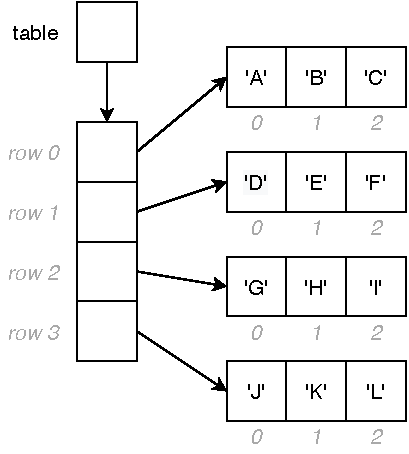
\includegraphics{RectArray.pdf}
\vspace{3em}


\quest{25 min}


\Q Run the program. What is the output of the following expressions?

\begin{enumerate}
\begin{multicols}{3}
\item \java{table.length}     \ans[2em]{4}
\item \java{table[0].length}  \ans[2em]{3}
\item \java{table[1][2]}      \ans[2em]{F}
\end{multicols}
\item \java{Arrays.toString(table)}
\hfill \ans[27em]{\jans{[[C@4dc63996, [C@d716361, [C@6ff3c5b5, [C@3764951d]}}
\end{enumerate}


\Q Based on the model, what is the data type of the following expressions? Please answer using Java syntax, for example: \java{String[]}

\begin{multicols}{3}
\begin{enumerate}
\item \java{table}
\ans[5em]{\jans{char[][]}}

\item \java{table[0]}
\ans[4em]{\jans{char[]}}

\item \java{table[1][2]}
\ans[4em]{\jans{char}}
\end{enumerate}
\end{multicols}


\Q \label{key1}
Explain the output of \java{Arrays.toString(table)}.
What exactly is stored in the array referenced by the variable \java{table}?

\begin{answer}[3em]
The output shows four memory addresses.
In other words, it's an array of references to other arrays (of characters).
\end{answer}


\Q Consider the expression \java{table[1][2]}.

\begin{enumerate}
\item Which index (1 or 2) represents the row number?    \ans[10em]{the first one}
\item Which index (1 or 2) represents the column number? \ans[10em]{the second one}
\end{enumerate}


\newpage

\Q What is the result of the following expressions?

\begin{multicols}{2}
\begin{enumerate}
\item \java{table[2][1]} \ans[8em]{H}
\item \java{table[0][0]} \ans[8em]{A}
\item \java{table[3][2]} \ans[8em]{L}
\item \java{table[2][3]} \ans[8em]{out of bounds}
\end{enumerate}
\end{multicols}


\vspace{1em}
\comment{Presenter: Implement your team's answers for the following questions in Model1.java, at the end of the main method. Make sure the code compiles and runs correctly.}


\Q Write three statements to print the first row of the table, one letter at a time.
The output should be \underline{\texttt{A~B~C~}} with a space after each letter.
%\textit{Hint:} Each line is the same except for one character.

\begin{answer}[5em]
\begin{javaans}
System.out.print(table[0][0] + " ");
System.out.print(table[0][1] + " ");
System.out.print(table[0][2] + " ");
\end{javaans}
\end{answer}


\Q Summarize the main difference in these three lines of code.

\begin{answer}[2em]
The second index changes from 0 to 1 to 2.
\end{answer}


\Q Rewrite your previous code using a \java{for} loop.
Name the loop variable \java{col} (instead of \java{i}).
Your code should work for any number of columns (not just 3).

\begin{answer}[5em]
\begin{javaans}
for (int col = 0; col < table[0].length; col++) {
    System.out.print(table[0][col] + " ");
}
\end{javaans}
\end{answer}


\Q Copy your answer to the previous question and paste it below two times.
Modify the code so that it prints row 2 and row 3.
Add \java{println} statements so that each row ends with a newline.

\begin{answer}[12em]
\begin{javaans}
for (int col = 0; col < table[1].length; col++) {
    System.out.print(table[1][col] + " ");
}
System.out.println();

for (int col = 0; col < table[2].length; col++) {
    System.out.print(table[2][col] + " ");
}
System.out.println();
\end{javaans}
\end{answer}


\Q Summarize the main differences in these two \java{for} loops.

\begin{answer}[2em]
The first index changes from 1 to 2, both in the loop condition and in the loop body.
\end{answer}


\Q \label{key2}
Rewrite your previous code using nested \java{for} loops.
Name the outer loop variable \java{row} and the inner loop variable \java{col}.
Your code should work for any number of rows and columns.

\begin{answer}[8em]
\begin{javaans}
for (int row = 0; row < table.length; row++) {
    for (int col = 0; col < table[row].length; col++) {
        System.out.print(table[row][col] + " ");
    }
    System.out.println();
}
\end{javaans}
\end{answer}


\Q How would you modify your code in the previous question to print only the top half of the table? (You may assume there is an even number of rows.)

\begin{answer}
Simply change the for loop header to be: \\[1ex]
\jans{for (int row = 0; row < table.length / 2; row++)}
\end{answer}
